% !TEX encoding = UTF-8 Unicode
%!TEX root = thesis.tex
% !TEX spellcheck = en-US
%%=========================================
\chapter{Summary and Conclusions} %% Summary, reflection, conclusion, yo dawg dis happened.
\label{chapterSummary}

%% THE FOLLOWING COMMENT IS REGARDING MASTER THESIS' AND SHOULD BE TREATED AS SUCH 
%% Here you give a summary of your your work and your results. This is like a management summary and should be written in a clear and easy language, without many difficult terms and without abbreviations. Everything you present here must be treated in more detail in the main report. You should not give any references to the report in the summary -- just explain what you have done and what you have found out. The Summary and Conclusions should be no more than two pages.

%% You may assume that you have got three minutes to present to the Rector of NTNU  what you have done and what you have found out as part of your thesis. (He is an intelligent person, but does not know much about your field of expertise.)

\section{Architecture}
\subsection{Architectural advantages}
In developing microservices, separation of responsibilities as a guiding principle has resulted in benefits like reuse of code and modularity. This is a notable advantage over other architectures, such as Server-Client and \acrlong{soa}. 
Server-Client architectures are generally monolithic, and over time in a production environment they grow unwieldy as new features are added, and old features are hard to replace without extensive code refactoring, because of internal backwards-compatibility.

\acrlong{soa} is an older architecture than microservices, though is in a way similar. Nevertheless, \acrshort{soa} has unclear and varying definitions and the architecture does not have the same overall guideline of separation of responsibilities as the microservice architecture. This leads to \acrshort{soa} often growing monolithic, as the responsibilities of each service grows, rather than being split into more services like with the microservice architecture.  

\subsection{Architectural disadvantages}
A complication with the microservice architecture is the separation of responsibilities. The group spent a while deciding which microservices to implement, and even throughout the project decisions were changed, as with the search service. 

Microservices, having large degrees of separation, also incur some communication overhead when using the exposed functionalities of each other. A related problem to this is how to share information that is common among services, without having redundancies. The group decided to give each service that needed one its own database, even though this incurred penalties with regards to redundancy. This was to ensure modularity and not having a service being replaced affect other services usage of stored data to a large extent. 

\section{Problems and solutions} 

\subsection {Time schedule}
\label{sub:timeSchedule}
Figure \ref{fig:wednesday} illustrates a typical Wednesday from 8:00 to 16:00, where a check mark indicates the team member being available, while unchecked indicates unavailable. Each row represents a team member. Most of the days in a week, including weekends, looked somewhat like this. The combined time schedules made it very hard to have regular meetings. Monday and Thursday afternoon were the only options which suited the entire group throughout most of the semester. Therefore all meetings with the client and supervisor were scheduled for these time slots. 

\begin{figure}[H]
    \centering
    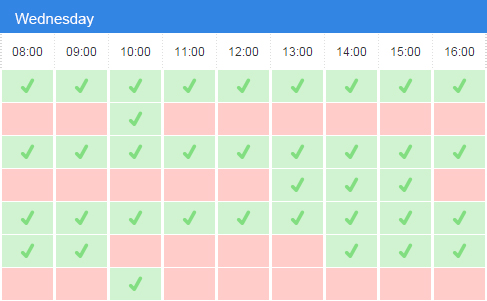
\includegraphics[scale=0.70]{fig/summary/wednesday}
    \caption{Example of our schedule. One row for each team member.}
    \label{fig:wednesday}
\end{figure}


\subsection{Abroad}
\noindent One of the group members had a part-time job in London the first half of the semester. This did not help the already troublesome schedule crash.
In addition, there was an excursion in March that three of the members were attending. This all meant a way of having stand-up meetings and exchanging information more frequently than the two meetings a week was needed. Geekbot was chosen for arranging online stand-up meetings. Communication is detailed in section \ref{sectionCommunicationTools}.

\subsection{Group member leaving}
At the beginning of the second iteration, a group member had to leave the course and the project for personal reasons. This meant that the group would go from seven people, down to six. The group worked around this by reassigning the workload to the remaining members. This announcement happened at a less unfortunate time, as the tasks for the second sprint had not yet been fully decided upon; planning for a six person group was relatively easy. 

This could of course have become problematic later on in the project if the total workload was larger than the reduced team could handle. Keeping in mind that the customer was more interested in a demonstration than the product features, scaling down functional requirements accordingly did not concern the customer much.

\section{Lessons learnt}

\subsection{Project organisation}

\paragraph{Schedules} Matching schedules is not a necessity for a project to succeed, but it makes the job a whole lot easier. Through planning and different tools, the problems were simplified, but with more similar schedules this could have been avoided in the first place. 

\paragraph{Development method} Looking back at the project, starting out with a more defined development method would have been beneficial and saved us some time. Agile development methods like Scrum work better when the team has a common background regarding development tools and how to use them. Digital Scrum boards, stand-up meetings, and other elements take time to learn and accustom to, and thus often benefit less than the required time investment for small projects.

\paragraph{Meetings} Even though it was not a huge problem, having more frequent meetings and work sessions would have improved the overall progression of the project early on. 

\subsection{Development}

\paragraph{Tools and frameworks} Learning to use tools and frameworks not familiar to the team may take more time than first anticipated. Thus, one should try to mostly use tools people are familiar with, unless the tool is required and there are no familiar alternatives.

\paragraph{Status} The status service could contain a cache of documentation and check if a newer version is available, to make sure documentation for a service is available even if the service is unavailable.

\paragraph{Front-end} The implemented front-end of the system is a bit too tightly coupled to be a true microservice. By splitting it up, or having different services provide their own front-end, this could have been achieved. This would require more work, despite being a nice possible addition to the project. 

\section{Conclusion}
The project started with some difficulties due to absence of one of the team members. This was handled by selecting an appropriate tool to facilitate team communication. This turned out to work quite well and had no major impact on the work flow. The roles and responsibilities of each team member were settled in a natural way, as each team member took on tasks that had been prioritised by the team. As the project evolved the different sub-teams worked on their part of the project and reported on the status during the weekly meetings. During the meetings people had the opportunity to share information and seek help on any problems encountered. 

Communication with the customer has been good overall, even though some more preparations could have been done beforehand by the team. All in all the project went smoothly and no major problems were encountered. 
%Any problems encountered along the way was taken care of in an efficient and effective way by the team, making the whole experience informative and interesting.

Even though the system is only a demonstration of microservices, it is a possibility that a third party might be interested in continuing working on the project. Therefore, steps have been taken to ensure that future developers can easily continue on the project if needed. The \acrshort{api} for every applicable microservice has been documented, so the services are easy to work with. If creating a replacement for a microservice is desirable, it is easy to find out which features require being implemented. A setup guide has been created to make it easy to deploy a new instance of the system. There are also tests for the services that can be used to validate future changes and make sure the system remains stable.

% forslag til oppsummerende setning: All in all the group felt that the requirements and goal defined at the start of the project ...somthing something ..

\section{Summary}

The project originated in the customer's expressed desire for a system implementation using microservices.
The group, through this project having implemented such a system, has to a large degree noticed many of the advantages that microservices are purported to have, which reflects many of the customer's hopes and expectations. %JA?
Overall, we feel that the requirements and goals outlined have been achieved to a satisfactory degree.
